\documentclass[tikz,border=2pt,11pt]{standalone}
\usetikzlibrary{arrows.meta}
\usetikzlibrary{decorations.pathreplacing}
\usetikzlibrary{calc}
\usetikzlibrary{patterns}
\usetikzlibrary{positioning}
\usepackage{amsmath}
\usepackage{amssymb}
\usepackage{mathrsfs}
\usepackage{xcolor}
\usepackage{graphicx}
\usepackage{tikz}
\newcommand{\R}{\mathbb R}
\newcommand{\C}{\mathbb C}
\newcommand{\Z}{\mathbb Z}
\newcommand{\N}{\mathbb N}
\newcommand{\PP}{\mathbb P}
\newcommand{\EE}{\mathbb E}
\newcommand{\Peta}{\mathbb P^{\eta}}
\newcommand{\Eeta}{\mathbb E^{\eta}}
\newcommand{\Esp}{\mathbb E_{\mathrm{sp}}}
\newcommand{\eps}{\varepsilon}
\newcommand{\om}{\omega}
\newcommand{\ind}{\mathbf 1}
\newcommand{\dd}{\mathrm d}
\newcommand{\ii}{\mathrm i}
\DeclareMathOperator{\diam}{diam}
\DeclareMathOperator{\dist}{dist}
\DeclareMathOperator{\supp}{supp}
\DeclareMathOperator{\Area}{Area}
\DeclareMathOperator{\Var}{Var}
\DeclareMathOperator{\Rea}{Re}
\DeclareMathOperator{\Ima}{Im}
\begin{document}
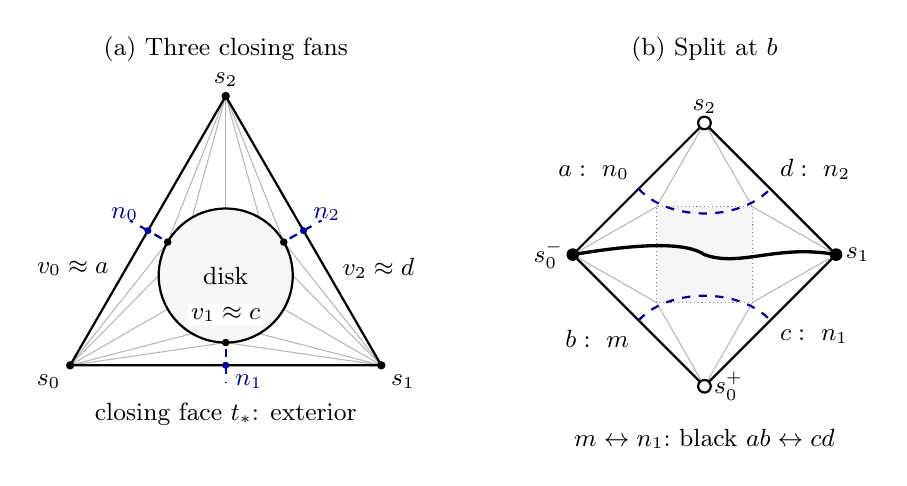
\begin{tikzpicture}[scale=.76, every node/.style={font=\small}]
\begin{scope}
 \coordinate (s0) at (-2.6,-1.5);
 \coordinate (s1) at (2.6,-1.5);
 \coordinate (s2) at (0,3);
 \fill[gray!7] (0,0) circle (1.12);
 \foreach \ang in {150,180,210,240,270}
   \draw[gray!55] (s0)--(\ang:1.12);
 \foreach \ang in {270,300,330,360,390}
   \draw[gray!55] (s1)--(\ang:1.12);
 \foreach \ang in {30,60,90,120,150}
   \draw[gray!55] (s2)--(\ang:1.12);
 \draw[thick] (s0)--(s1)--(s2)--cycle;
 \draw[thick] (0,0) circle (1.12);
 \foreach \pos in {150,270,30}{
   \fill (\pos:1.12) circle (1.8pt);
 }
 \node[anchor=east,fill=white,inner sep=1pt] at (-1.9,.12) {$v_0\approx a$};
 \node[fill=white,inner sep=1pt] at (0,-.65) {$v_1\approx c$};
 \node[anchor=west,fill=white,inner sep=1pt] at (1.9,.12) {$v_2\approx d$};
 \fill (s0) circle (2pt) node[below left] {$s_0$};
 \fill (s1) circle (2pt) node[below right] {$s_1$};
 \fill (s2) circle (2pt) node[above] {$s_2$};
 \node at (0,0) {disk};
 \draw[blue!65!black,dashed,thick] (-1.07,.62)--(-1.60,.92);
 \draw[blue!65!black,dashed,thick] (0,-1.23)--(0,-1.80);
 \draw[blue!65!black,dashed,thick] (1.07,.62)--(1.60,.92);
 \fill[blue!65!black] (-1.3,.75) circle (1.7pt)
   node[above left] {$n_0$};
 \fill[blue!65!black] (0,-1.5) circle (1.7pt)
   node[below right] {$n_1$};
 \fill[blue!65!black] (1.3,.75) circle (1.7pt)
   node[above right] {$n_2$};
 \node[align=center] at (0,-2.32) {closing face $t_*$\text{: exterior}};
 \node at (0,3.78) {(a) Three closing fans};
\end{scope}
\begin{scope}[xshift=8.0cm,yshift=.35cm]
 \coordinate (l) at (-2.2,0);
 \coordinate (r) at (2.2,0);
 \coordinate (u) at (0,2.2);
 \coordinate (v) at (0,-2.2);
 \fill[gray!7] (-.8,-.8) rectangle (.8,.8);
 \draw[gray!55] (l)--(-.8,.8) (l)--(-.8,-.8)
   (v)--(-.8,-.8) (v)--(.8,-.8)
   (r)--(.8,-.8) (r)--(.8,.8)
   (u)--(.8,.8) (u)--(-.8,.8);
 \draw[thick] (l)--(v)--(r)--(u)--cycle;
 \draw[gray,densely dotted] (-.8,-.8) rectangle (.8,.8);
 \draw[very thick] (l) .. controls (-1,.20) and (-.3,.20) .. (0,0)
    .. controls (.6,-.22) and (1.2,.18) .. (r);
 \draw[blue!65!black,dashed,thick] (-1.1,-1.1)
    .. controls (-.6,-.55) and (.6,-.55) .. (1.1,-1.1);
 \draw[blue!65!black,dashed,thick] (-1.1,1.1)
    .. controls (-.6,.55) and (.6,.55) .. (1.1,1.1);
 \foreach \p in {l,r} \fill (\p) circle (3pt);
 \foreach \p in {u,v} \draw[fill=white,thick] (\p) circle (3pt);
 \node[left] at (l) {$s_0^-$};
 \node[right] at (r) {$s_1$};
 \node[above] at (u) {$s_2$};
 \node[right] at (v) {$s_0^+$};
 \node[above left] at (-1.1,1.1) {$a:\ n_0$};
 \node[below left] at (-1.1,-1.1) {$b:\ m$};
 \node[below right] at (1.1,-1.1) {$c:\ n_1$};
 \node[above right] at (1.1,1.1) {$d:\ n_2$};
 \node[align=center] at (0,-3.08) {$m\leftrightarrow n_1$:\ black $ab\leftrightarrow cd$};
 \node at (0,3.43) {(b) Split at $b$};
\end{scope}
\end{tikzpicture}
\end{document}
